\documentclass{article}
\usepackage[utf8]{inputenc}
\usepackage{graphicx}
\graphicspath{ {./} }
\title{Assignment2}
\author{Jiapeng Zhang}
\date{May 2021}

\begin{document}

\maketitle

\section{Question 1}
In Question 1, two different methods to generate derivatives were implemented and by comparing its error relative to the analytical results with a loglog plot to determine which one is the most optimal.

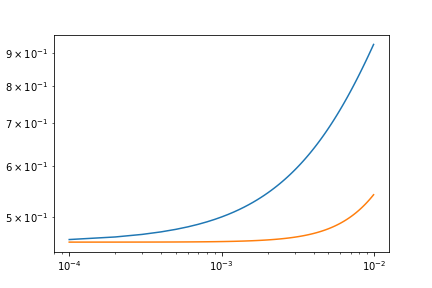
\includegraphics[scale=0.8]{Question_1.png}

From the above plot, the error for the second method is significantly smaller than the first method. The slope from the above plot represents the error increasing speed.

\section{Question 2}
For {c=x+yi|-2<x,y<2}, by parsing through a large number of points within this region, each point will either diverge into unrepresentable in python (i.e. NaN+NaNi) or stay bounded with in a certain region. To plot the corresponding points, different coordinates were recorded in different list. For the diverging points, the number of iterations when they reach NaN+NaNi is also recorded in a different set of list.

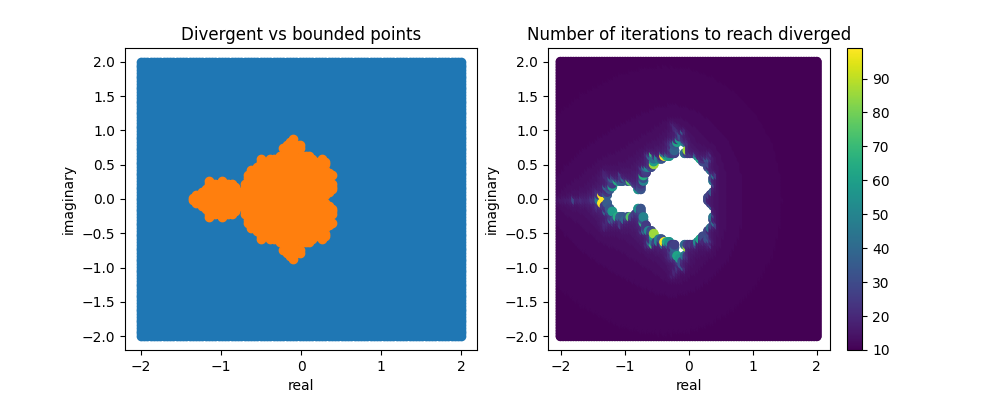
\includegraphics[scale=0.5]{Question_2.png}

From above plots, the bounded points form a Mandelbrot set. Also, most of the diverging points will reach NaN+NaNi after around 10 times of iterations.

\section{Question 3}
SIR model represents the likely trend when a new contagious non-lethal virus firstly surface without any treatment, depending on the force of the virus and the susceptibility of the herd. Here, four sets of two parameters are simulated to see the trend of each one of them.The four sets of parameters $(\beta,\gamma)=[(0.5,0.2),(0.4,0.2),(0.4,0.3),(0.5,0.3)]$. Here are $\beta$ is larger than $\gamma$, which means that even though the force of the virus is strong but not all individuals will be infected. It depends on the immunity of the individuals, its contact towards the virus and other factors. The difference between $\beta$ and $\gamma$ accounts for such uncertainty. 

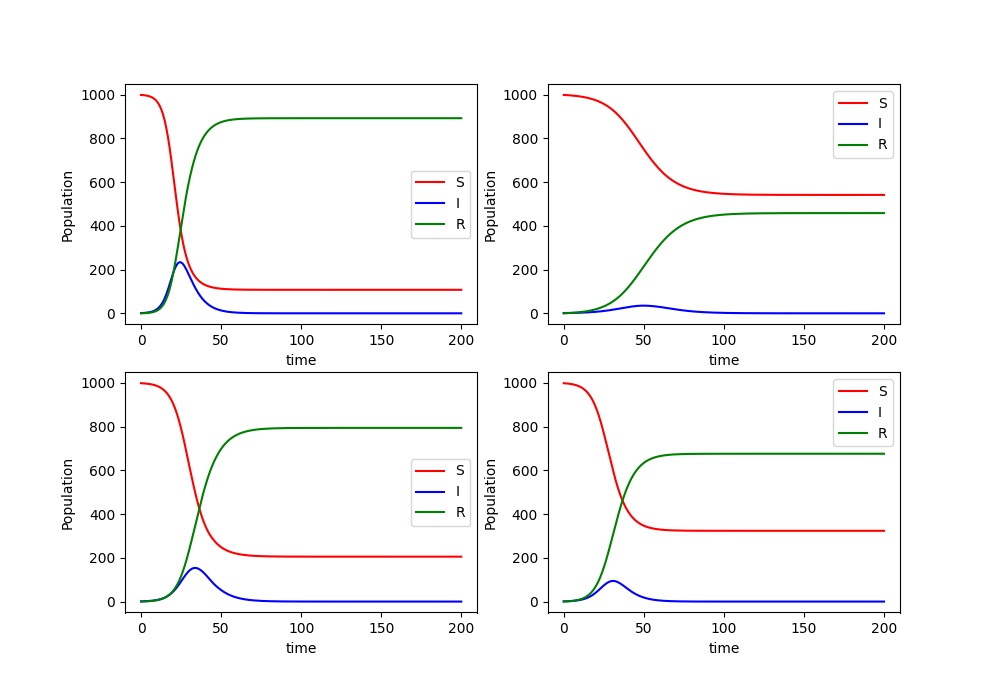
\includegraphics[scale=0.4]{Question_3(a).png}

From the figures above, even though they vary largely from one another, but the common thing is that not all susceptible individuals are infected when the new stability is achieved.

\section{Bonus}

For death, there should be a new parameter $\alpha$ to determine to death rate. Since the death can only come from the infected, the differential equation for death rate should be as follow:
\begin{equation}
    \large\frac{dD}{dt} =\alpha I
\end{equation}
Now, because the total population is set to remain unchanged meaning $\frac{dN}{dt}=0$ and the increased infected should deduct the death rate. Therefore the infected equation should be modified as follow:
\begin{equation}
    \large\frac{dI}{dt}=-\frac{\beta SI}{N} -\gamma I -\alpha I
\end{equation}

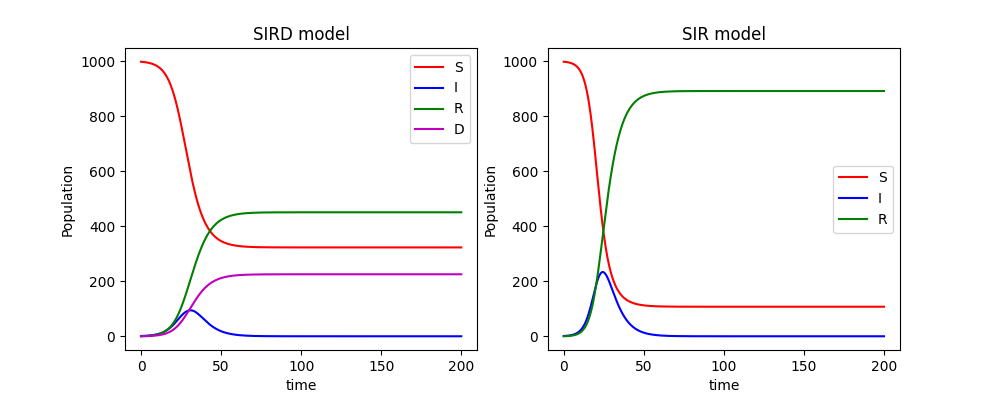
\includegraphics[scale=0.5]{Question_3(b).png}
This new equation has the same parameter with the first set from SIR model, plus a death rate parameter $\alpha=0.1$. From the figures above, the time it takes to re-establish stability does not change. However, due to the death factor, the maximum infected population is lower. The remaining susceptible population is much larger than SIR model, because it took fewer people to reach herd immunity.
\end{document}
